\documentclass[compress]{beamer}
\mode<presentation>
{
 \usetheme{Vilanova}
}

\usepackage[french]{babel}

\usepackage[utf8]{inputenc}

\usepackage{times}
\usepackage[T1]{fontenc}

\usepackage{amsfonts}
\usepackage{amsmath}
\usepackage{amssymb}
\usepackage{tikz}
\usepackage{eurosym}
%\usepackage{url}
\usepackage[normal]{subfigure}
\newcommand{\goodgap}{%
	\hspace{\subfigtopskip}%
	\hspace{\subfigbottomskip}}



%\newtheorem{definition}{Definition}

\title{Corrections géométriques}

\subtitle{Modèles de capteur et projections cartographiques} % (optional)


\author
{jordi.inglada@cesbio.cnes.fr}
\normalsize

\institute[Cesbio] % (optional, but mostly needed)
{\textsc{Centre d'Études Spatiales de la Biosphère, Toulouse, France}}

\date{}

\pgfdeclareimage[height=96mm,width=128mm]{background}{fondsClairSansLogo}
\setbeamertemplate{background}{\pgfuseimage{background}}
\pgfdeclareimage[height=0.6cm]{logoIncrust}{logoIncrust}
\pgfdeclareimage[height=0.5cm]{logo_cesbio}{logo_cesbio}
\logo{
\begin{tabular}{lp{0.25\textwidth}lp{0.25\textwidth}r}
\href{http://www.cesbio.ups-tlse.fr/}{\pgfuseimage{logo_cesbio}}
&&\footnotesize{AUF - Marrakech 2011}&&
\href{http://www.orfeo-toolbox.org}{\pgfuseimage{logoIncrust}}\\
\end{tabular}
}


\subject{Image geometry in ORFEO Toolbox}




% Delete this, if you do not want the table of contents to pop up at
% the beginning of each subsection:
\AtBeginSubsection[]
{
  \begin{frame}<beamer>
    \frametitle{Outline}
    \tableofcontents[currentsection,currentsubsection]
  \end{frame}
}




% If you wish to uncover everything in a step-wise fashion, uncomment
% the following command: 

%\beamerdefaultoverlayspecification{<+->}
\begin{document}

\begin{frame}
  \titlepage
  \begin{center}
{\tiny Ce contenu est dérivé de la formation \href{http://www.orfeo-toolbox.org/packages/PragmaticRemoteSensing-handout.pdf}{``Pragmatic Remote
  Sensing''} dispensée par J. Inglada et E. Christophe en juillet 2010
  dans le cadre du colloque IGARSS. Il est mis à disposition selon les termes de la licence :\\
Creative Commons Paternité – Partage à l’Identique 3.0 non transcrit.} \href{http://creativecommons.org/licenses/by-sa/3.0/}{\includegraphics[width=0.05\textwidth]{/home/inglada/Dev/GH/IGARSS2010/Tutorial/Slides/Ressources/CC-licence.png}}    
  \end{center}
\end{frame}


\section*{Introduction}

\begin{frame}

  \frametitle{Introduction}
  \hspace*{-1cm}
  \begin{tikzpicture}[scale=0.165]
    \tiny
    \draw[fill=black!10] (-1,-12) rectangle (75,17);
     \foreach \x in {5,...,1}
       \draw[fill=red] (\x,\x) rectangle +(4,4);
     \node[fill=black!10, text width= 1.5cm] (InputSeries) at
       (4,-1) {Série d'images};
     \pause
     \draw[->,thick] (9,5) --  +(3,0);
     \pause
     \draw[fill=black!30,rounded corners=2pt] (12.2,3) rectangle +(6,4);
     \node[text width= 0.8cm] (SensorModel) at (15,5) {Modèle capteur};
     \pause
     \draw[fill=red!30] (1,-10) rectangle +(4,4);
     \node[fill=black!10, text width= 1.2cm] (DEM) at
       (5,-11) {MNT};
     \pause
     \draw[->,thick] (3,-5.5) --  ++(0,3) -- ++(12,0) -- ++(0,5);
     \pause
     \draw[->,thick] (18.5,5) --  +(3,0);
     \pause
     \foreach \x in {5,...,1}
       \draw[fill=blue,xshift=600pt] (\x,\x) rectangle +(4,4);
     \node[fill=black!10, text width= 2.8cm] (GeoRefSeries) at
       (28,-1) {Géo-référencement};
\pause
      

       \draw[->,thick] (25.5,8.5) --  +(0,3);
       
     \draw[fill=black!30,rounded corners=2pt] (22,12) rectangle +(8.5,4);
     \node[text width= 1.5cm] (HomPoExtr) at (27,14) {Points Homologues};

     \draw[->,thick] (21.5,14) --  +(-2.5,0);

     \draw[fill=black!30,rounded corners=2pt] (11,12) rectangle +(8,4);
     \node[text width= 1.3cm] (BBAdj) at (15.5,14) {Spatio triangulation};

     \draw[->,thick] (15,11.5) --  +(0,-4);

     \pause
      \draw[->,thick] (30,5) --  +(3,0);
      \pause
     \draw[fill=black!30,rounded corners=2pt] (33.2,2.5) rectangle +(6,4.5);
     \node[text width= 0.7cm] (FineRegistration) at (36,4.9) {Recalage fin};
     \pause

     
     \draw[->,thick] (39.5,5) --  +(3,0);
     \pause
     \foreach \x in {5,...,1}
       \draw[fill=green,xshift=1200pt] (\x,\x) rectangle +(4,4);
     \node[fill=black!10, text width= 1.8cm] (RegistSeries) at
       (47,-1) {Série recalée};
     \pause
     \draw[->,thick] (36,2) --  ++(0,-10) -- ++(-30,0);

     \pause
      \draw[->,thick] (52,5) --  +(3,0);
      \pause
     \draw[fill=black!30,rounded corners=2pt] (55.2,2.5) rectangle +(6,4.5);
     \node[text width= 0.7cm] (CartoProjection) at (57.5,4.9)
          {Projection Carto};
     \pause

     
     \draw[->,thick] (61.5,5) --  +(3,0);
     \pause
     \foreach \x in {5,...,1}
       \draw[fill=yellow,xshift=1810pt] (\x,\x) rectangle +(4,4);
     \node[fill=black!10, text width= 1.95cm] (CartoSeries) at
       (68,-1) {Ortho-images};
     
       
  \end{tikzpicture}
\end{frame}

%% \begin{frame}
%%   \frametitle{Introduction}
%%  \begin{block}{How to register image series}
%%  \begin{itemize}
%%  \item Sensor models and bundle-block adjustment
%%  \item Homologous point extraction
%%  \item Fine registration
%%  \end{itemize}
%%  \end{block}
%%  \begin{block}{How to measure the quality}
%%  \begin{itemize}
%%  \item Choosing the reference
%%  \item Quality measures
%%  \end{itemize}
%%  \end{block}
%%  \end{frame}


\section[Modèles]{Modèles de capteur}


\begin{frame}
  \frametitle{Modèles de capteur}

  \framesubtitle{Définition}
Transformation de coordonnées entre l'image issue du capteur $(l,c)$
et les coordonnées au sol $(X,Y)$ pour chaque pixel :
\pause
\begin{displaymath}
  \begin{array}{cc}
    Direct & \\
    X = f_x(l,c,h,\vec\theta) & Y = f_y(l,c,h,\vec\theta)\\
     & \\ \pause
    Inverse & \\
    l = g_l(X,Y,h,\vec\theta) & c = g_c(X,Y,h,\vec\theta)
  \end{array}
\end{displaymath}
\pause
Où $\vec\theta$ est l'ensemble de paramètres décrivant le capteur et
la géométrie d'acquisition.\\
\pause
L'élévation de chaque point (MNT) doit être connue.
  
\end{frame}

\begin{frame}
  \frametitle{Modèles de capteur}

  \framesubtitle{Types de modèles}
  \begin{itemize}
    \item Modèles physiques
      \begin{itemize}
	\item Rigoureux, complexes, équations fortement non-linéaires
	\item Difficiles à inverser
	\item Les paramètres ont une signification physique
	\item Specifiques à chaque capteur
      \end{itemize}
    \item Modèles analytiques génériques
      \begin{itemize}
	\item Ex: polynomiaux, fractions rationnelles, etc.
	\item Moins précis
	\item Faciles à mettre en ouevre
	\item Les paramètres peuvent ne pas avoir de signification physique
      \end{itemize}
  \end{itemize}

\end{frame}

\begin{frame}
  \frametitle{Modèles de capteur}

  \framesubtitle{L'approche OTB}
  \begin{itemize}
    \item Utilisation de {\em factories} : les modèles sont générés
      automatiquement en utilisant les méta-données des images
    \item Modèles disponibles
      \begin{itemize}
	\item Fractions rationnelles : Quickbird, Ikonos, WorldView-2
	\item Modèles physiques : SPOT5
	\item Radar : ERS, ASAR, Radarsat, Cosmo, TerraSAR-X, Palsar
      \end{itemize}
  \end{itemize}
\end{frame}


\begin{frame}
\frametitle{La main à la pâte}
\begin{enumerate}
\item Monteverdi : Ouvrir une image Quickbird en géométrie capteur
\item Afficher l'image
\item Observer comment les coordonnées géographiques sont recalculées
  quand le curseur se déplace
\end{enumerate}
\end{frame}

\begin{frame}
  \frametitle{Modèles de capteur}

  \framesubtitle{Utilisation : ortho-rectification}
  \begin{enumerate}
    \item Lecture des méta-données image et création du modèle avec
      les bons paramètres
  \item Définition de la ROI en coordonnées sol (c'est la matrice de
    pixels de sortie)
  \item Balayer les pixels de coordonnées $(X,Y)$ :
    \begin{enumerate}
      \item Obtenir $h$ à partir du MNT
      \item Calculer $(c,l) = G(X,Y,h,\vec\theta)$
      \item Interpoler les valeurs des pixels si $(c,l)$ ne sont pas
        des valeurs entières
    \end{enumerate}
  \end{enumerate}
\end{frame}

\begin{frame}
\frametitle{La main à la pâte}
\begin{enumerate}
\item Monteverdi: Geometry $\rightarrow$ Orthorectification
\item Choisir l'image à ortho-rectifier
\item Choisir les paramètres
\item Sauvegarder le résultat
\item Répéter pour la 2ème image
\item Afficher les 2 images ensemble
\end{enumerate}
\end{frame}


\begin{frame}
  \frametitle{Modèles de capteur}
  \framesubtitle{Limites de l'approche}

  \begin{itemize}
    \item Un géo-référencement précis nécessite :
      \begin{itemize}
	\item Un MNT précis
	\item Des paramètres capteur sans erreur, $\vec\theta$
      \end{itemize}
    \item Pour les séries multi-temporelles d'images on a besoin de
      \alert{recalage fin} :
      \begin{itemize}
      \item Précision sous-pixellique
      \item Pour chaque pixel de la scène
      \end{itemize}
    \item Les MNT et les méta-données capteur ne fournissent pas cette
      précision.
    \item Solution : utilisation de l'information redondante entre les
      images de la série.
  \end{itemize}
\end{frame}

\section{Optimizations}
\subsection[BBA]{Bundle-block adjustment}

\begin{frame}
  \frametitle{Bundle-block adjustment}
  \framesubtitle{Problem position}
  \begin{columns}[T]
\column{.5\textwidth}
  \begin{itemize}
    \item The image series is geo-referenced (using the available DEM,
    and the prior sensor parameters).
    \item We assume that homologous points (GCPs, etc.) can be easily
    obtained from the geo-referenced series : $HP_i = (X_i,Y_i,h_i)$
    \item For each image, and each point, we can write:
    $(l_{ij},c_{ij}) = G_j(X_i,Y_i,h_i,\vec\theta_j)$
  \end{itemize}
\column{.5\textwidth}
\begin{tikzpicture}[scale=0.15]
\draw[fill=yellow!20] (-5.5,-15.5) rectangle (5.5,-5.5);
    \draw[step=0.5, gray, very thin] (-5.5,-15.5) grid (5.5,-5.5);

    \draw[fill=green!20,rotate=10] (-15.5,0.5) rectangle (-5.5,10.5);
    \draw[step=0.5, gray, very thin,rotate=10] (-15.5,0.5) grid
    (-5.5,10.5);

    \draw[fill=blue!20,rotate=-10] (5.5,0.5) rectangle (15.5,10.5);
    \draw[step=0.5, gray, very thin,rotate=-10] (5.5,0.5) grid
    (15.5,10.5);

    \pause
    \draw[fill=red!70] (1,-11) circle (0.2);
    \pause
    \draw (1,-11) .. controls +(30:1cm) and +(60:1cm) .. (-10,7);
    \pause
    \draw[fill=red!70] (-10,7) circle (0.2);
    \pause
    \node (eq1) at (-12.2,-4) {$\scriptstyle{G_1(X_i,Y_i,h_i,\vec\theta_1)}$};
    \pause
    \draw (1,-11) .. controls +(-30:1cm) and +(-60:1cm) .. (10,7);
    \pause
    \draw[fill=red!70] (10,7) circle (0.2);
    \pause
    \node (eq2) at (7.2,-3) {$\scriptstyle{G_2(X_i,Y_i,h_i,\vec\theta_2)}$};
    
\end{tikzpicture}
\begin{itemize}
      \item Everything is known.
\end{itemize}
  \end{columns}
\end{frame}

\begin{frame}
  \frametitle{Bundle-block adjustment}
  \framesubtitle{Model refinement}
  \begin{itemize}
    \item If we define $\vec\theta_j^R = \vec\theta_j +
    \vec{\Delta\theta_j}$ as the refined parameters,
    $\vec{\Delta\theta_j}$ are the unknowns of the model refinement
    problem.
    \item We have much more equations than unknowns if enough HPs are
    found.
    \item We solve using non-linear least squares estimation.
      \begin{itemize}
	\item The derivatives of the sensor model with respect to its
	parameters are needed.
      \end{itemize}
  \end{itemize}
  
\end{frame}

\begin{frame}
  \frametitle{Hands On}
  \framesubtitle{Manually register 2 images}
\vspace*{-0.6cm}
\small
  \begin{itemize}
  \item Monteverdi: Geometry $\rightarrow$ Homologous points extraction
  \item Select 2 images with a common region
  \item The GUI lets you select a transformation
  \item You can select homologous points in the zoom images and add
    them to the list
  \item When several homologous points are available, you can evaluate
    the transform
  \item Once the transform is evaluated, you can use the {\em guess}
    button to predict the position in the moving image of a point
    selected in the fixed image
  \item The GUI displays the parameters of the transform estimated as
    well as individual error for each point and the MSE
  \item You can remove from the list the points with higher error
  \end{itemize}
\end{frame}

%% \subsection{Fine registration}
%% \begin{frame}
%% \frametitle{Why fine registration?}
%% \begin{itemize}
%%   \item Homologous points have been used to refine the sensor model
%%   \item Residual misregistrations exist because of:
%%     \begin{itemize}
%%       \item DEM errors
%%       \item Sensor model approximations
%%       \item Surface objects (high resolution imagery)
%%     \end{itemize}
%%   \item We want to find the homologous point
%%     \begin{itemize}
%%       \item of every pixel in the reference image
%%       \item with sub-pixel accuracy
%%     \end{itemize}
%%   \item This is called \alert{disparity map}
%% \end{itemize}
%% \end{frame}

%% \begin{frame}
%%   \frametitle{Fine registration (under development)}
%%   \begin{tikzpicture}[scale=0.35]
%%     \draw[fill=green!20] (5,5) rectangle (15,15);
%%     \draw[step=0.5, gray, very thin] (5,5) grid (15,15);
%%     \node (Reference) at (10,3) {Reference Image};

%%     \draw[fill=blue!20] (25,5) rectangle (35,15);
%%     \draw[step=0.5, gray, very thin] (25,5) grid (35,15);
%%     \node (Reference) at (30,3) {Secondary Image};
%%     \pause
%%     \draw[fill=red!60] (7,12) circle (0.2);
%%     \draw[fill=red!60] (27,12) circle (0.2);
%%     \node (CPs) at (20,14) {\tiny Candidate points};
%%     \pause
%%     \draw[thick] (6.5,11.5) rectangle +(1,1);
%%     \node (EW) at (20,13) {\tiny Estimation window};
%%     \pause
%%     \draw[fill=gray, opacity=0.5] (25,10) rectangle +(4,4);
%%     \node (SW) at (20,12) {\tiny Search window};
%%     \pause
%%     \draw[thick] (25,13) rectangle +(1,1);
%%     \node (SEW) at (20,11) {\tiny Similarity estimation};
%%     \pause
%%     \draw[red,->] (25.5,13.5) --  ++(3,0) -- ++(0,-0.5) -- ++(-3,0) -- ++(0,-0.5) --++(3,0) -- ++(0,-0.5)  ;
%%     \node (OPT) at (20,10) {\tiny Similarity optimization};
%%     \pause
%%     \draw[fill=green!60] (28,10.5) circle (0.2);
%%     \node (OPTF) at (20,9) {\tiny Optimum};
%%     \pause
%%     \draw[blue!80,->] (27,12) -- (28,10.5);
%%     \node (Deltas) at (20,8) {$\scriptstyle{\Delta_x,\Delta_y}$};
    
%%   \end{tikzpicture}
%%   \end{frame}

%% \section{Map projections}
%% \begin{frame}
%%   \frametitle{Map projections}

%%   \framesubtitle{What is a map projection}
%% Gives the relationship between geographic $(X,Y)$ and cartographic $(x,y)$ coordinates.
%% \pause
%% \begin{displaymath}
%%   \begin{array}{cc}
%%     Forward & \\
%%     x = f_x(X,Y,\vec\alpha) & y = f_y(X,Y,\vec\alpha)\\
%%      & \\ \pause
%%     Inverse & \\
%%     X = g_X(x,y,\vec\alpha) & Y = g_y(x,y,\vec\alpha)
%%   \end{array}
%% \end{displaymath}
%% \pause
%% Where $\vec\alpha$ is the set of parameters of a given map projection.\\
  
%% \end{frame}

%% \begin{frame}
%%   \frametitle{Map projections}

%%   \framesubtitle{Types of map projections}
%%   \begin{itemize}
%%     \item OTB implements most of the OSSIM ones:
%%       \begin{itemize}
%% 	\item 30 map projections are available among which: UTM,
%% 	  TransMercator, LambertConformalConic, etc.
%% 	  %% Albers, AzimEquDist, Bng, Bonne, Cadrg, Cadrg, Cassini,
%% %% 	  CylEquArea, Eckert4, Eckert6, Gnomonic,
%% %% 	  LambertConformalConic, Llxy, EquDistCyl, Mercator, Miller,
%% %% 	  Mollweid, NewZealandMapGrid, ObliqueMercator, OrthoGraphic,
%% %% 	  PolarStereo, PolyconicInverseProjection, Sinusoidal,
%% %% 	  SpaceObliqueMercator, Stereographic, TransCylEquArea,
%% %% 	  TransMercator, Ups, Utm, VanDerGrinten.
%%       \end{itemize}
%%     \item For any Xyz projection the \texttt{otb::XyzForwardProjection} and
%%       the \texttt{otb::XyzInverseProjection} are available.
%%     \item Change of projections can be implemented by using one
%%       forward, one inverse and the \texttt{otb::CompositeTransform} class.
%%     \item One-step ortho-registration can be implemented by
%%       combining a sensor model and a map projection.
%%   \end{itemize}

%% \end{frame}

%% \begin{frame}
%%   \frametitle{Hands On}
%%   \framesubtitle{Changing image projections}
%%   \begin{itemize}
%%   \item Monteverdi: Geometry $\rightarrow$ Reproject Image
%%   \item Select an orthorectified image as input image
%%   \item Select the projection you want as output
%%   \item Save/Quit
%%   \end{itemize}
%% \end{frame}

%% \begin{frame}
%%   \frametitle{Hands On}
%%   \framesubtitle{Apply the geometry of one image to another}
%%   \begin{itemize}
%%   \item Monteverdi: Geometry $\rightarrow$ Superimpose 2 Images
%%   \item Select any as image image to reproject
%%   \item Select an orthorectified image as reference image
%%     \begin{itemize}
%%     \item Make sure the 2 images have a common region!
%%     \end{itemize}
%%   \item Use the same DEM (if any) as for the ortho-rectified image 
%%   \item Save/Quit
%%   \end{itemize}
%% \end{frame}


%% \begin{frame}[c]
%% \frametitle{As a conclusion}
%% \begin{enumerate}
%%   \item Use a good sensor model if it exists
%%   \item Use a good DEM if you have it\label{demItem}
%%   \item Improve you sensor parameters after a first geo-referencing
%%   pass\label{bbaItem}
%%   \item Fine-register your series
%% %%     \begin{itemize}
%% %%       \item Choose your reference
%% %%       \item Choose a suited similarity measure
%% %%       \item Use a good interpolator
%% %%       \item Get your disparity map (series)
%% %%       \item Re-sample your images
%% %%       \item Improve your DEM and goto \ref{demItem}
%% %%     \end{itemize}
%%   \item Use a map projection
%%     \end{enumerate}
%% \begin{itemize}
%%   \item All these steps can be performed
%%   with OTB/Monteverdi.
%%   \item Sensor model + map projection using a DEM are available as a
%%   one-step filter in OTB.
  
%% \end{itemize}


%% \end{frame}


%% \begin{frame}[c]
%% \frametitle{ORFEO Toolbox}
%% \framesubtitle{... is not a black box!}
%% \begin{center}
%%   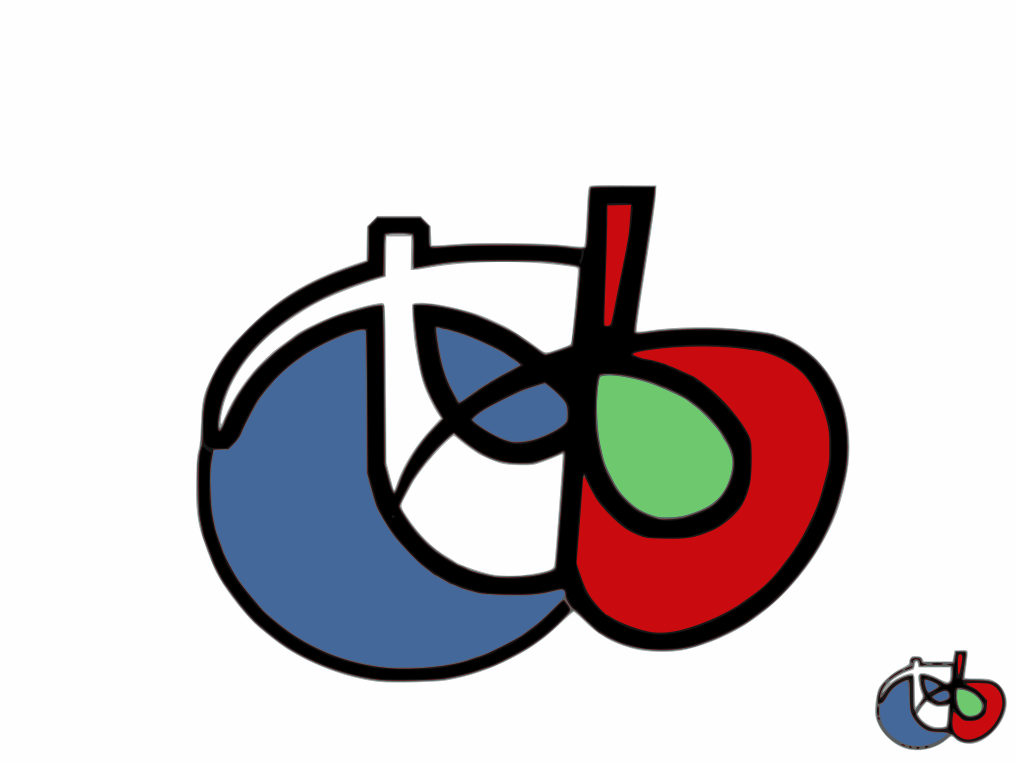
\includegraphics[width=0.2\textwidth]{logoVectoriel}
%% \end{center}
%% \begin{itemize}
%%   \item CNES' free image analysis software
%%    \begin{itemize}
%%      \item Segmentation
%%      \item Feature extraction
%%      \item Registration
%%      \item ...
%%    \end{itemize}
%%   \item Download here \href{http://smsc.cnes.fr/PLEIADES/A_prog_accomp.htm}{http://smsc.cnes.fr/PLEIADES/A\_prog\_accomp.htm}.%{\pgfuseimage{logoIncrust}}.
%% \end{itemize}
%% \end{frame}
\end{document}
